
\section{Introduction}
This report has been written for the Master Artificial Intelligence course Autonomous Agents. This report will contain the answers, motivation and explanation for our implementations of the tasks we had to accomplish in our third assignment for this course. These tasks were centered around the topic of `Multi-Agent Planning and Learning'.

\subsection{The environment} \label{sec:environment}
In all tasks there is assumed to be a grid world (of $11 \times 11$) with at least one predator and a prey in it. The agents can both move one tile forward each iteration. The direction they take (or if they move at all) is affected by probabilities (their policies). If they move over the edge of the grid they end up at the opposing side of the grid. We are focused on improving the decisions of all the agents, the predator(s) and the prey. 

\subsection{The state space representation} \label{sec:stateSpaceIntro}
In this assignment, we used the efficient state space representation that we also used in the previous Assignment for the learning algorithms. To give a good understanding of our learning algorithms, which were built again using this efficient state space representation, we will once again explain how this representation works.

Figure \ref{fig:statespaceSymm} illustrates that there is a symmetry in the default state space, and thus that there were relatively much values redundantly computed.
By using this symmetry in the default state space a much smaller state space was achieved. 

Each state represents a distance between the prey and predator. These are represented in the lower left diagonal of a matrix, in which the $x$-axis is the relative horizontal distance in the MDP and the $y$-axis the relative vertical distance in the MDP. This matrix is shown in Figure \ref{fig:NewStateRep}. Combinations of positions of prey and predator for which the horizontal and vertical distances are equal are now treated equivalent. 
Also two combinations for which the horizontal distance in one equals the vertical distance in the other and vice versa are considered equal. In order to navigate through this state space different actions are required. These are: \textit{horizontal retreat, horizontal approach, vertical retreat, vertical approach}, as illustrated in Figure \ref{fig:statespaceSymm}, and of course the action \textit{wait}. When interacting with the environment these actions are converted into corresponding actions in the real world. This only requires the relative direction of the prey (which is always located at the centre, regardless of its coordinates) with respect to the predator. This is computed by using the difference in location of the prey and predator on the $x$- and $y$-axis.

\begin{figure}[ht]
\centering
\subfigure[The $11 \times 11$ grid divided into eight symmetric pieces, with the corresponding possible moves which are also symmetric.]{
    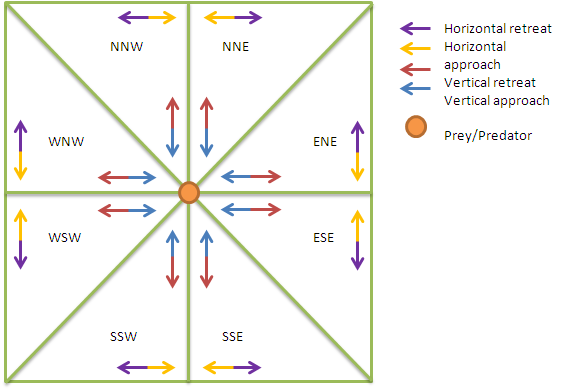
\includegraphics[width=0.5\textwidth]{statespaceSymm.png}
    \label{fig:statespaceSymm}
}
\subfigure[Colormap of $V$-values, the brighter the color the higher the corresponding $V$-value. The prey is always located on the (1, 1) coordinate in this state representation.]{
    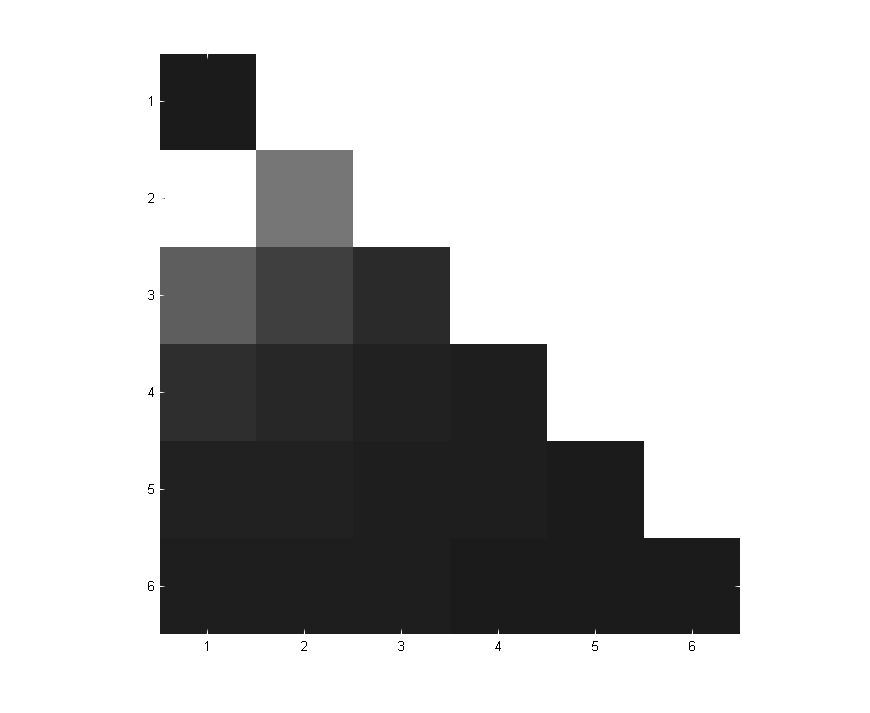
\includegraphics[width=0.4\textwidth]{VMatrixNewStateRep.png}
    \label{fig:NewStateRep}
}
\caption{Illustration of the symmetry and corresponding values of the new state space representation}
\label{fig:statespaceIll}
\end{figure}

Note that this state representation works only for two agents (here we talked about one prey and one predator). For Independent Q-Learning (see Section \ref{sec:IQL}), in which more agents will be used, we will require a more extensive state space. That state space is, however, still built upon this one.

\subsection{Implementation details}
This report will not be about our exact code and implementation details. However, a class diagram of our code is provided alongside the source code.
